\documentclass{article}

\usepackage{fancyhdr}
\usepackage{extramarks}
\usepackage{amsmath}
\usepackage{amsthm}
\usepackage{amssymb}
\usepackage{amsfonts}
\usepackage{tikz}
\usepackage{physics}
\usepackage[plain]{algorithm}
\usepackage{algpseudocode}
\usepackage{hyperref}

\usetikzlibrary{automata,positioning}

%
% Basic Document Settings
%

\topmargin=-0.45in
\evensidemargin=0in
\oddsidemargin=0in
\textwidth=6.5in
\textheight=9.0in
\headsep=0.25in

\linespread{1.1}

\pagestyle{fancy}
\lhead{\hmwkAuthorName}
\chead{\hmwkClass\ : \hmwkTitle}
\rhead{\firstxmark}
\lfoot{\lastxmark}
\cfoot{\thepage}

\renewcommand\headrulewidth{0.4pt}
\renewcommand\footrulewidth{0.4pt}

\setlength\parindent{0pt}

%
% Create Problem Sections
%
\newcommand{\be}{\begin{equation}}
\newcommand{\ee}{\end{equation}}
\newcommand{\bes}{\begin{equation*}}
\newcommand{\ees}{\end{equation*}}
\newcommand{\bea}{\begin{flalign*}}
\newcommand{\eea}{\end{flalign*}}


\newcommand{\enterProblemHeader}[1]{
    \nobreak\extramarks{}{Problem \arabic{#1} continued on next page\ldots}\nobreak{}
    \nobreak\extramarks{Problem \arabic{#1} (continued)}{Problem \arabic{#1} continued on next page\ldots}\nobreak{}
}

\newcommand{\exitProblemHeader}[1]{
    \nobreak\extramarks{Problem \arabic{#1} (continued)}{Problem \arabic{#1} continued on next page\ldots}\nobreak{}
    \stepcounter{#1}
    \nobreak\extramarks{Problem \arabic{#1}}{}\nobreak{}
}

\setcounter{secnumdepth}{0}
\newcounter{partCounter}
\newcounter{homeworkProblemCounter}
\setcounter{homeworkProblemCounter}{1}
\nobreak\extramarks{Problem \arabic{homeworkProblemCounter}}{}\nobreak{}

%
% Homework Problem Environment
%
% This environment takes an optional argument. When given, it will adjust the
% problem counter. This is useful for when the problems given for your
% assignment aren't sequential. See the last 3 problems of this template for an
% example.
%
\newenvironment{homeworkProblem}[1][-1]{
    \ifnum#1>0
        \setcounter{homeworkProblemCounter}{#1}
    \fi
    \section{Problem \arabic{homeworkProblemCounter}}
    \setcounter{partCounter}{1}
    \enterProblemHeader{homeworkProblemCounter}
}{
    \exitProblemHeader{homeworkProblemCounter}
}

%
% Homework Details
%   - Title
%   - Due date
%   - Class
%   - Section/Time
%   - Instructor
%   - Author
%

\newcommand{\hmwkTitle}{Homework\ \#1}
\newcommand{\hmwkDueDate}{Due on 14th January, 2019}
\newcommand{\hmwkClass}{Dynamical Systems}
\newcommand{\hmwkClassTime}{}
\newcommand{\hmwkClassInstructor}{}
\newcommand{\hmwkAuthorName}{\textbf{Aditya Vijaykumar}}

%
% Title Page
%

\title{
    %\vspace{2in}
    \textmd{\textbf{\hmwkClass:\ \hmwkTitle}}\\
    \normalsize\vspace{0.1in}\small{\hmwkDueDate\ }\\
%    \vspace{3in}
}

\author{\hmwkAuthorName}
\date{}

\renewcommand{\part}[1]{\textbf{\large Part \Alph{partCounter}}\stepcounter{partCounter}\\}

%
% Various Helper Commands
%

% Useful for algorithms
\newcommand{\alg}[1]{\textsc{\bfseries \footnotesize #1}}

% For derivatives
\newcommand{\deriv}[1]{\frac{\mathrm{d}}{\mathrm{d}x} (#1)}

% For partial derivatives
\newcommand{\pderiv}[2]{\frac{\partial}{\partial #1} (#2)}

% Integral dx
\newcommand{\dx}{\mathrm{d}x}

% Alias for the Solution section header
\newcommand{\solution}{\textbf{\large Solution}}

% Probability commands: Expectation, Variance, Covariance, Bias
\newcommand{\E}{\mathrm{E}}
\newcommand{\Var}{\mathrm{Var}}
\newcommand{\Cov}{\mathrm{Cov}}
\newcommand{\Bias}{\mathrm{Bias}}

\begin{document}

\maketitle
(\textbf{Acknowledgements} - I would like to thank Divya Jagannathan for discussions.)
\\

\begin{homeworkProblem}
	\begin{equation}
	\dot{x} = x^{1/3} \implies \dfrac{dx}{x^{1/3}} = dt \implies \dfrac{2}{3} \qty(x^{2/3} - x_0^{2/3}) = t \implies x(t) = \qty(x_0^{2/3} + \dfrac{3}{2}t)^{3/2}
	\label{eq1}
	\end{equation}
	For $ x_0 = 0 $, we have $ x(t) = \qty(\dfrac{3t}{2})^{3/2} $. As the function $ f(y) = y^{3/2} $ is only defined for $ y \ge 0 $, this solution has maximum interval of existence $ t \in [0, \infty)$. For $ x_0 = 0 $, we also have the trivial solution $ x(t) = 0 $ which has maximum interval of existence $ t \in (-\infty, \infty) $. So there are at least two distinct solutions for $ x_0=0 $. One can also imagine patching up the above solutions at origin and forming other possible solutions.
	\\
	
	For the case where $ x_0 \ne 0 $, we are only left with [\ref{eq1}]. As $ x_0^{2/3} > 0, \forall x_0 \ne 0 $, the maximal interval of existence for $ x(t) $ is $ \left[ -\dfrac{2}{3} x_0^{2/3},\infty\right) $.
	
	If we try to solve the problem numerically, we only get the trivial solution $ x(t) = 0  $ for $ x_0 = 0 $.
\end{homeworkProblem}









\begin{homeworkProblem}
	\textbf{Part (a)}\\
	\begin{equation*}
	\dot{x} = x ( x^2 - 1)
	\end{equation*}
	For $ x_0 = 0,1,-1 $, $ x(t) = 0, 1, -1 $ respectively is a solution for all times.
	\begin{align*}
	\therefore \dfrac{dx}{x ( x-1 )(x+1)} &= dt\\
	\therefore - \dfrac{dx}{x} +\dfrac{1}{2}\qty[\dfrac{dx}{x+1} + \dfrac{dx}{x-1}] &= dt\\
	\dfrac{1}{2} \log \abs{\dfrac{x_0^2(x^2 -1)}{x^2 (x_0^2 - 1)}} &= t \\
	\dfrac{(x^2 -1)}{x^2 } &= \pm \dfrac{x_0^2 - 1}{x_0^2}e^{2t}\\
	x(t) &= \sqrt{\dfrac{1}{1  \pm {\dfrac{x_0^2 - 1}{x_0^2}} e^{2t}}}
	\end{align*}
	We take only the $ - $ sign in the above expression as the $ + $ sign does not satisfy the initial condition.
	\begin{equation*}
	x(t) =\dfrac{x_0}{\abs{x_0}}  \sqrt{\dfrac{1}{1  - {\dfrac{x_0^2 - 1}{x_0^2}} e^{2t}}}
	\end{equation*}
	where the $ \dfrac{x_0}{\abs{x_0}} $ has been multiplied to take care of sign.
	For the problem to have the above solution, one must have,
	\begin{align*}
	1 - {\dfrac{x_0^2 - 1}{x_0^2}} e^{2t} > 0 &\implies t < -\dfrac{1}{2} \log {\dfrac{x_0^2 - 1}{x_0^2}} \qq{if}  x_0^2 > 1 \\
	&\qq{and} t \in (-\infty, \infty) \qq{if} x_0^2 < 1
	\end{align*}
	
	\begin{figure}[!h]
	\caption{Q2 (a)}
	\centering
	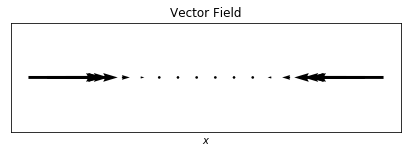
\includegraphics[scale=0.6]{2a_1.png}
	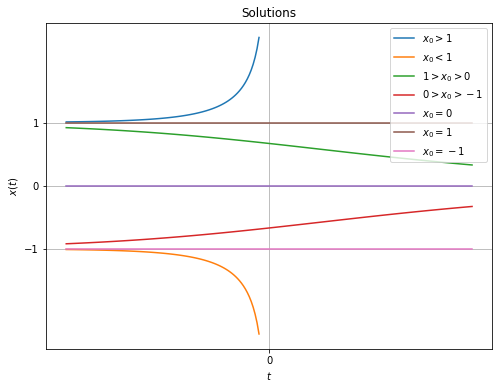
\includegraphics[scale=0.45]{2a_3.png}
	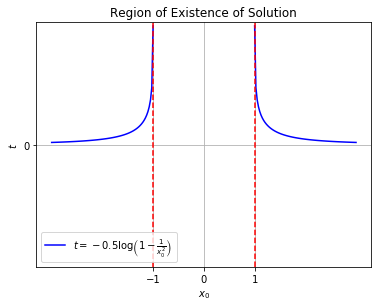
\includegraphics[scale=0.6]{2a_2.png}
	\end{figure}
	
	\textbf{Part (b)}\\
	\begin{equation*}
	\dot{x} = -x^3
	\end{equation*}
	The above equation has the trivial solution $ x(t) = 0; \forall t $ for $ x_0 = 0 $. We proceed to find solutions for other values of $ x_0 $.
	\begin{align*}
	\dot{x} = - x^3 \implies -\dfrac{dx}{x^3} = dt &\implies \eval{\dfrac{1}{2x^2}}_{x_0}^{x} = t \implies \dfrac{1}{x^2} = \dfrac{1}{x_0^2} + 2t\\
	\implies &x = + \dfrac{ x_0}{\sqrt{1 + 2 x_0^2 t}}
	\end{align*}
	The above solution will exist for $ t > -\dfrac{1}{2x_0^2} ; x_0 \ne 0$. The region of existence is also plotted below.
	
	\begin{figure}[h]
		\caption{Q2 (b)}
		\centering
		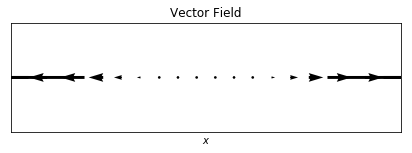
\includegraphics[scale=0.6]{2b_3.png}
		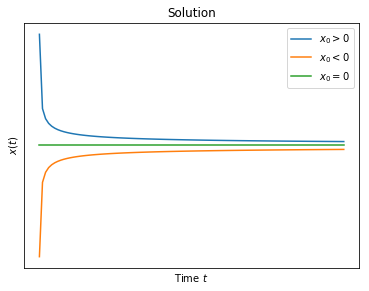
\includegraphics[scale=0.6]{2b_1.png}
		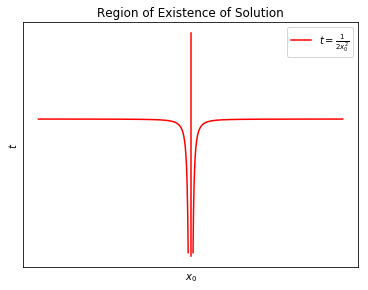
\includegraphics[scale=0.6]{2b_2.png}
		
	\end{figure}
	
	\textbf{Part (c)}\\
	Given that 
	\begin{align*}
	E &= \dfrac{x_2^2}{2} + \dfrac{x_1^2}{2} - \dfrac{x_1^4}{4} \\
	\dot{E} &= x_2 \dot{x}_2 + x_1 \dot{x}_1 - {\dot{x}_1 x_1^3}\\
	&= -x_1 x_2 + x_1^3 x_2 + x_1 x_2 - x_2 x_1^3 = 0\\
	E&= constant
	\end{align*}
	Hence the system as defined in the question is a Hamiltonian system. Now we can proceed to analytically solve this equation,
	\begin{align*}
	\dfrac{\dot{x}_1^2}{2} + \dfrac{x_1^2}{2} - \dfrac{x_1^4}{4} = E \\
	\implies \dot{x}_1 = \sqrt{2 E + \dfrac{x_1^4 }{2}-  x_1^2}\\
	\implies x = \int dx_1 \sqrt{2 E + \dfrac{x_1^4 }{2}-  x_1^2} 
	\end{align*}
	
	\begin{figure}[!h]
	\caption{Q2 (c)}
	\centering
	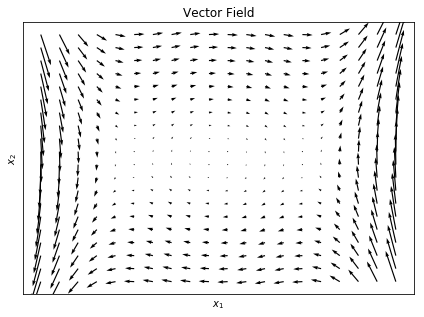
\includegraphics[scale=0.6]{2c_1.png}
	\end{figure}
\end{homeworkProblem}

\begin{homeworkProblem}
	\textit{Solved completely in the Jupyter Notebook.}
\end{homeworkProblem}









\begin{homeworkProblem}
	One definition of religion is \footnote{Dictionary of Philosophy of Religion, Taliaferro \& Marty 2010} :-
	
	\textit{A religion involves a communal, transmittable body of teachings and prescribed practices about an ultimate, sacred reality or state of being \textbf{that calls for reverence or awe}, a body which guides its practitioners into what it describes as a saving, illuminating or emancipatory relationship to this reality through a personally transformative life of prayer, ritualized meditation, and/or moral practices like repentance and personal regeneration.}
	\\
	
	One can argue whether this definition is really general, but I think to first order religions like Hinduism, Islam and Christianity agree with this definition.
	\\
	
	If one is pedantic about it, science, unlike religion, is only a recently coined term and has been in vogue only since the 19th Century\footnote{https://plato.stanford.edu/entries/religion-science/\#WhatScieWhatReli}. The most accepted definition of a scientific hypothesis was given by Karl Popper in 1959, w\textit{hich, in short, states that \textit{scientific hypotheses should in-principle be falsifiable}. There is no reference made to an absolute authority of science}, which then is the most striking difference between science and religion.
	\\
	
	Note that this is not to say there aren't any similarities between science and religion - science communities also have cults like religion.
	
\end{homeworkProblem}

\end{document}
